% Created by tikzDevice version 0.12.3.1 on 2021-04-04 17:56:12
% !TEX encoding = UTF-8 Unicode
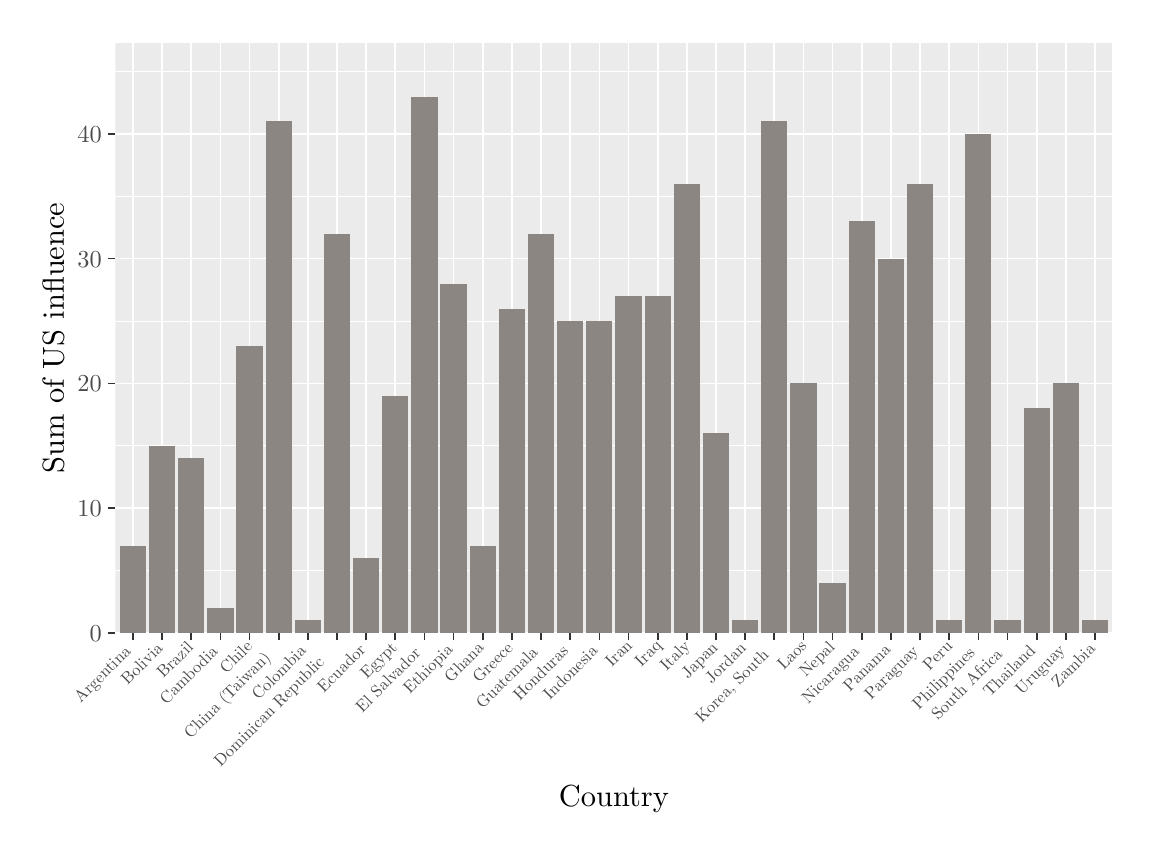
\begin{tikzpicture}[x=1pt,y=1pt]
\definecolor{fillColor}{RGB}{255,255,255}
\path[use as bounding box,fill=fillColor,fill opacity=0.00] (0,0) rectangle (397.48,289.08);
\begin{scope}
\path[clip] (  0.00,  0.00) rectangle (397.48,289.08);
\definecolor{drawColor}{RGB}{255,255,255}
\definecolor{fillColor}{RGB}{255,255,255}

\path[draw=drawColor,line width= 0.6pt,line join=round,line cap=round,fill=fillColor] (  0.00,  0.00) rectangle (397.48,289.08);
\end{scope}
\begin{scope}
\path[clip] ( 31.71, 70.39) rectangle (391.98,283.58);
\definecolor{fillColor}{gray}{0.92}

\path[fill=fillColor] ( 31.71, 70.39) rectangle (391.98,283.58);
\definecolor{drawColor}{RGB}{255,255,255}

\path[draw=drawColor,line width= 0.3pt,line join=round] ( 31.71, 92.93) --
	(391.98, 92.93);

\path[draw=drawColor,line width= 0.3pt,line join=round] ( 31.71,138.00) --
	(391.98,138.00);

\path[draw=drawColor,line width= 0.3pt,line join=round] ( 31.71,183.07) --
	(391.98,183.07);

\path[draw=drawColor,line width= 0.3pt,line join=round] ( 31.71,228.14) --
	(391.98,228.14);

\path[draw=drawColor,line width= 0.3pt,line join=round] ( 31.71,273.21) --
	(391.98,273.21);

\path[draw=drawColor,line width= 0.6pt,line join=round] ( 31.71, 70.39) --
	(391.98, 70.39);

\path[draw=drawColor,line width= 0.6pt,line join=round] ( 31.71,115.47) --
	(391.98,115.47);

\path[draw=drawColor,line width= 0.6pt,line join=round] ( 31.71,160.54) --
	(391.98,160.54);

\path[draw=drawColor,line width= 0.6pt,line join=round] ( 31.71,205.61) --
	(391.98,205.61);

\path[draw=drawColor,line width= 0.6pt,line join=round] ( 31.71,250.68) --
	(391.98,250.68);

\path[draw=drawColor,line width= 0.6pt,line join=round] ( 38.03, 70.39) --
	( 38.03,283.58);

\path[draw=drawColor,line width= 0.6pt,line join=round] ( 48.57, 70.39) --
	( 48.57,283.58);

\path[draw=drawColor,line width= 0.6pt,line join=round] ( 59.10, 70.39) --
	( 59.10,283.58);

\path[draw=drawColor,line width= 0.6pt,line join=round] ( 69.64, 70.39) --
	( 69.64,283.58);

\path[draw=drawColor,line width= 0.6pt,line join=round] ( 80.17, 70.39) --
	( 80.17,283.58);

\path[draw=drawColor,line width= 0.6pt,line join=round] ( 90.70, 70.39) --
	( 90.70,283.58);

\path[draw=drawColor,line width= 0.6pt,line join=round] (101.24, 70.39) --
	(101.24,283.58);

\path[draw=drawColor,line width= 0.6pt,line join=round] (111.77, 70.39) --
	(111.77,283.58);

\path[draw=drawColor,line width= 0.6pt,line join=round] (122.31, 70.39) --
	(122.31,283.58);

\path[draw=drawColor,line width= 0.6pt,line join=round] (132.84, 70.39) --
	(132.84,283.58);

\path[draw=drawColor,line width= 0.6pt,line join=round] (143.38, 70.39) --
	(143.38,283.58);

\path[draw=drawColor,line width= 0.6pt,line join=round] (153.91, 70.39) --
	(153.91,283.58);

\path[draw=drawColor,line width= 0.6pt,line join=round] (164.44, 70.39) --
	(164.44,283.58);

\path[draw=drawColor,line width= 0.6pt,line join=round] (174.98, 70.39) --
	(174.98,283.58);

\path[draw=drawColor,line width= 0.6pt,line join=round] (185.51, 70.39) --
	(185.51,283.58);

\path[draw=drawColor,line width= 0.6pt,line join=round] (196.05, 70.39) --
	(196.05,283.58);

\path[draw=drawColor,line width= 0.6pt,line join=round] (206.58, 70.39) --
	(206.58,283.58);

\path[draw=drawColor,line width= 0.6pt,line join=round] (217.12, 70.39) --
	(217.12,283.58);

\path[draw=drawColor,line width= 0.6pt,line join=round] (227.65, 70.39) --
	(227.65,283.58);

\path[draw=drawColor,line width= 0.6pt,line join=round] (238.18, 70.39) --
	(238.18,283.58);

\path[draw=drawColor,line width= 0.6pt,line join=round] (248.72, 70.39) --
	(248.72,283.58);

\path[draw=drawColor,line width= 0.6pt,line join=round] (259.25, 70.39) --
	(259.25,283.58);

\path[draw=drawColor,line width= 0.6pt,line join=round] (269.79, 70.39) --
	(269.79,283.58);

\path[draw=drawColor,line width= 0.6pt,line join=round] (280.32, 70.39) --
	(280.32,283.58);

\path[draw=drawColor,line width= 0.6pt,line join=round] (290.86, 70.39) --
	(290.86,283.58);

\path[draw=drawColor,line width= 0.6pt,line join=round] (301.39, 70.39) --
	(301.39,283.58);

\path[draw=drawColor,line width= 0.6pt,line join=round] (311.92, 70.39) --
	(311.92,283.58);

\path[draw=drawColor,line width= 0.6pt,line join=round] (322.46, 70.39) --
	(322.46,283.58);

\path[draw=drawColor,line width= 0.6pt,line join=round] (332.99, 70.39) --
	(332.99,283.58);

\path[draw=drawColor,line width= 0.6pt,line join=round] (343.53, 70.39) --
	(343.53,283.58);

\path[draw=drawColor,line width= 0.6pt,line join=round] (354.06, 70.39) --
	(354.06,283.58);

\path[draw=drawColor,line width= 0.6pt,line join=round] (364.60, 70.39) --
	(364.60,283.58);

\path[draw=drawColor,line width= 0.6pt,line join=round] (375.13, 70.39) --
	(375.13,283.58);

\path[draw=drawColor,line width= 0.6pt,line join=round] (385.66, 70.39) --
	(385.66,283.58);
\definecolor{fillColor}{RGB}{139,134,130}

\path[fill=fillColor] ( 33.29, 70.39) rectangle ( 42.77,101.94);

\path[fill=fillColor] ( 43.83, 70.39) rectangle ( 53.31,138.00);

\path[fill=fillColor] ( 54.36, 70.39) rectangle ( 63.84,133.49);

\path[fill=fillColor] ( 75.43, 70.39) rectangle ( 84.91,174.06);

\path[fill=fillColor] ( 96.50, 70.39) rectangle (105.98, 74.90);

\path[fill=fillColor] (107.03, 70.39) rectangle (116.51,214.62);

\path[fill=fillColor] (117.57, 70.39) rectangle (127.05, 97.44);

\path[fill=fillColor] (128.10, 70.39) rectangle (137.58,156.03);

\path[fill=fillColor] (149.17, 70.39) rectangle (158.65,196.59);

\path[fill=fillColor] (159.70, 70.39) rectangle (169.18,101.94);

\path[fill=fillColor] (170.24, 70.39) rectangle (179.72,187.58);

\path[fill=fillColor] (180.77, 70.39) rectangle (190.25,214.62);

\path[fill=fillColor] (191.31, 70.39) rectangle (200.79,183.07);

\path[fill=fillColor] (201.84, 70.39) rectangle (211.32,183.07);

\path[fill=fillColor] (212.38, 70.39) rectangle (221.86,192.09);

\path[fill=fillColor] (222.91, 70.39) rectangle (232.39,192.09);

\path[fill=fillColor] (233.44, 70.39) rectangle (242.92,232.65);

\path[fill=fillColor] (254.51, 70.39) rectangle (263.99, 74.90);

\path[fill=fillColor] (243.98, 70.39) rectangle (253.46,142.51);

\path[fill=fillColor] ( 64.90, 70.39) rectangle ( 74.38, 79.41);

\path[fill=fillColor] (265.05, 70.39) rectangle (274.53,255.19);

\path[fill=fillColor] (275.58, 70.39) rectangle (285.06,160.54);

\path[fill=fillColor] (296.65, 70.39) rectangle (306.13,219.13);

\path[fill=fillColor] (286.12, 70.39) rectangle (295.60, 88.42);

\path[fill=fillColor] (307.18, 70.39) rectangle (316.66,205.61);

\path[fill=fillColor] (328.25, 70.39) rectangle (337.73, 74.90);

\path[fill=fillColor] (338.79, 70.39) rectangle (348.27,250.68);

\path[fill=fillColor] (317.72, 70.39) rectangle (327.20,232.65);

\path[fill=fillColor] (138.64, 70.39) rectangle (148.12,264.20);

\path[fill=fillColor] (359.86, 70.39) rectangle (369.34,151.52);

\path[fill=fillColor] ( 85.96, 70.39) rectangle ( 95.44,255.19);

\path[fill=fillColor] (370.39, 70.39) rectangle (379.87,160.54);

\path[fill=fillColor] (349.32, 70.39) rectangle (358.80, 74.90);

\path[fill=fillColor] (380.92, 70.39) rectangle (390.40, 74.90);
\end{scope}
\begin{scope}
\path[clip] (  0.00,  0.00) rectangle (397.48,289.08);
\definecolor{drawColor}{gray}{0.30}

\node[text=drawColor,anchor=base east,inner sep=0pt, outer sep=0pt, scale=  0.88] at ( 26.76, 67.36) {0};

\node[text=drawColor,anchor=base east,inner sep=0pt, outer sep=0pt, scale=  0.88] at ( 26.76,112.44) {10};

\node[text=drawColor,anchor=base east,inner sep=0pt, outer sep=0pt, scale=  0.88] at ( 26.76,157.51) {20};

\node[text=drawColor,anchor=base east,inner sep=0pt, outer sep=0pt, scale=  0.88] at ( 26.76,202.58) {30};

\node[text=drawColor,anchor=base east,inner sep=0pt, outer sep=0pt, scale=  0.88] at ( 26.76,247.65) {40};
\end{scope}
\begin{scope}
\path[clip] (  0.00,  0.00) rectangle (397.48,289.08);
\definecolor{drawColor}{gray}{0.20}

\path[draw=drawColor,line width= 0.6pt,line join=round] ( 28.96, 70.39) --
	( 31.71, 70.39);

\path[draw=drawColor,line width= 0.6pt,line join=round] ( 28.96,115.47) --
	( 31.71,115.47);

\path[draw=drawColor,line width= 0.6pt,line join=round] ( 28.96,160.54) --
	( 31.71,160.54);

\path[draw=drawColor,line width= 0.6pt,line join=round] ( 28.96,205.61) --
	( 31.71,205.61);

\path[draw=drawColor,line width= 0.6pt,line join=round] ( 28.96,250.68) --
	( 31.71,250.68);
\end{scope}
\begin{scope}
\path[clip] (  0.00,  0.00) rectangle (397.48,289.08);
\definecolor{drawColor}{gray}{0.20}

\path[draw=drawColor,line width= 0.6pt,line join=round] ( 38.03, 67.64) --
	( 38.03, 70.39);

\path[draw=drawColor,line width= 0.6pt,line join=round] ( 48.57, 67.64) --
	( 48.57, 70.39);

\path[draw=drawColor,line width= 0.6pt,line join=round] ( 59.10, 67.64) --
	( 59.10, 70.39);

\path[draw=drawColor,line width= 0.6pt,line join=round] ( 69.64, 67.64) --
	( 69.64, 70.39);

\path[draw=drawColor,line width= 0.6pt,line join=round] ( 80.17, 67.64) --
	( 80.17, 70.39);

\path[draw=drawColor,line width= 0.6pt,line join=round] ( 90.70, 67.64) --
	( 90.70, 70.39);

\path[draw=drawColor,line width= 0.6pt,line join=round] (101.24, 67.64) --
	(101.24, 70.39);

\path[draw=drawColor,line width= 0.6pt,line join=round] (111.77, 67.64) --
	(111.77, 70.39);

\path[draw=drawColor,line width= 0.6pt,line join=round] (122.31, 67.64) --
	(122.31, 70.39);

\path[draw=drawColor,line width= 0.6pt,line join=round] (132.84, 67.64) --
	(132.84, 70.39);

\path[draw=drawColor,line width= 0.6pt,line join=round] (143.38, 67.64) --
	(143.38, 70.39);

\path[draw=drawColor,line width= 0.6pt,line join=round] (153.91, 67.64) --
	(153.91, 70.39);

\path[draw=drawColor,line width= 0.6pt,line join=round] (164.44, 67.64) --
	(164.44, 70.39);

\path[draw=drawColor,line width= 0.6pt,line join=round] (174.98, 67.64) --
	(174.98, 70.39);

\path[draw=drawColor,line width= 0.6pt,line join=round] (185.51, 67.64) --
	(185.51, 70.39);

\path[draw=drawColor,line width= 0.6pt,line join=round] (196.05, 67.64) --
	(196.05, 70.39);

\path[draw=drawColor,line width= 0.6pt,line join=round] (206.58, 67.64) --
	(206.58, 70.39);

\path[draw=drawColor,line width= 0.6pt,line join=round] (217.12, 67.64) --
	(217.12, 70.39);

\path[draw=drawColor,line width= 0.6pt,line join=round] (227.65, 67.64) --
	(227.65, 70.39);

\path[draw=drawColor,line width= 0.6pt,line join=round] (238.18, 67.64) --
	(238.18, 70.39);

\path[draw=drawColor,line width= 0.6pt,line join=round] (248.72, 67.64) --
	(248.72, 70.39);

\path[draw=drawColor,line width= 0.6pt,line join=round] (259.25, 67.64) --
	(259.25, 70.39);

\path[draw=drawColor,line width= 0.6pt,line join=round] (269.79, 67.64) --
	(269.79, 70.39);

\path[draw=drawColor,line width= 0.6pt,line join=round] (280.32, 67.64) --
	(280.32, 70.39);

\path[draw=drawColor,line width= 0.6pt,line join=round] (290.86, 67.64) --
	(290.86, 70.39);

\path[draw=drawColor,line width= 0.6pt,line join=round] (301.39, 67.64) --
	(301.39, 70.39);

\path[draw=drawColor,line width= 0.6pt,line join=round] (311.92, 67.64) --
	(311.92, 70.39);

\path[draw=drawColor,line width= 0.6pt,line join=round] (322.46, 67.64) --
	(322.46, 70.39);

\path[draw=drawColor,line width= 0.6pt,line join=round] (332.99, 67.64) --
	(332.99, 70.39);

\path[draw=drawColor,line width= 0.6pt,line join=round] (343.53, 67.64) --
	(343.53, 70.39);

\path[draw=drawColor,line width= 0.6pt,line join=round] (354.06, 67.64) --
	(354.06, 70.39);

\path[draw=drawColor,line width= 0.6pt,line join=round] (364.60, 67.64) --
	(364.60, 70.39);

\path[draw=drawColor,line width= 0.6pt,line join=round] (375.13, 67.64) --
	(375.13, 70.39);

\path[draw=drawColor,line width= 0.6pt,line join=round] (385.66, 67.64) --
	(385.66, 70.39);
\end{scope}
\begin{scope}
\path[clip] (  0.00,  0.00) rectangle (397.48,289.08);
\definecolor{drawColor}{gray}{0.30}

\node[text=drawColor,rotate= 45.00,anchor=base east,inner sep=0pt, outer sep=0pt, scale=  0.60] at ( 37.57, 63.30) {Argentina};

\node[text=drawColor,rotate= 45.00,anchor=base east,inner sep=0pt, outer sep=0pt, scale=  0.60] at ( 49.18, 64.37) {Bolivia};

\node[text=drawColor,rotate= 45.00,anchor=base east,inner sep=0pt, outer sep=0pt, scale=  0.60] at ( 60.11, 64.77) {Brazil};

\node[text=drawColor,rotate= 45.00,anchor=base east,inner sep=0pt, outer sep=0pt, scale=  0.60] at ( 69.06, 63.18) {Cambodia};

\node[text=drawColor,rotate= 45.00,anchor=base east,inner sep=0pt, outer sep=0pt, scale=  0.60] at ( 81.45, 65.05) {Chile};

\node[text=drawColor,rotate= 45.00,anchor=base east,inner sep=0pt, outer sep=0pt, scale=  0.60] at ( 88.07, 61.13) {China (Taiwan)};

\node[text=drawColor,rotate= 45.00,anchor=base east,inner sep=0pt, outer sep=0pt, scale=  0.60] at (100.94, 63.47) {Colombia};

\node[text=drawColor,rotate= 45.00,anchor=base east,inner sep=0pt, outer sep=0pt, scale=  0.60] at (107.45, 59.44) {Dominican Republic};

\node[text=drawColor,rotate= 45.00,anchor=base east,inner sep=0pt, outer sep=0pt, scale=  0.60] at (122.44, 63.90) {Ecuador};

\node[text=drawColor,rotate= 45.00,anchor=base east,inner sep=0pt, outer sep=0pt, scale=  0.60] at (133.81, 64.73) {Egypt};

\node[text=drawColor,rotate= 45.00,anchor=base east,inner sep=0pt, outer sep=0pt, scale=  0.60] at (142.31, 62.70) {El Salvador};

\node[text=drawColor,rotate= 45.00,anchor=base east,inner sep=0pt, outer sep=0pt, scale=  0.60] at (153.95, 63.81) {Ethiopia};

\node[text=drawColor,rotate= 45.00,anchor=base east,inner sep=0pt, outer sep=0pt, scale=  0.60] at (165.20, 64.52) {Ghana};

\node[text=drawColor,rotate= 45.00,anchor=base east,inner sep=0pt, outer sep=0pt, scale=  0.60] at (175.69, 64.47) {Greece};

\node[text=drawColor,rotate= 45.00,anchor=base east,inner sep=0pt, outer sep=0pt, scale=  0.60] at (184.67, 62.92) {Guatemala};

\node[text=drawColor,rotate= 45.00,anchor=base east,inner sep=0pt, outer sep=0pt, scale=  0.60] at (195.70, 63.41) {Honduras};

\node[text=drawColor,rotate= 45.00,anchor=base east,inner sep=0pt, outer sep=0pt, scale=  0.60] at (206.28, 63.46) {Indonesia};

\node[text=drawColor,rotate= 45.00,anchor=base east,inner sep=0pt, outer sep=0pt, scale=  0.60] at (218.80, 65.44) {Iran};

\node[text=drawColor,rotate= 45.00,anchor=base east,inner sep=0pt, outer sep=0pt, scale=  0.60] at (229.35, 65.47) {Iraq};

\node[text=drawColor,rotate= 45.00,anchor=base east,inner sep=0pt, outer sep=0pt, scale=  0.60] at (239.65, 65.23) {Italy};

\node[text=drawColor,rotate= 45.00,anchor=base east,inner sep=0pt, outer sep=0pt, scale=  0.60] at (249.71, 64.75) {Japan};

\node[text=drawColor,rotate= 45.00,anchor=base east,inner sep=0pt, outer sep=0pt, scale=  0.60] at (259.91, 64.42) {Jordan};

\node[text=drawColor,rotate= 45.00,anchor=base east,inner sep=0pt, outer sep=0pt, scale=  0.60] at (268.12, 62.10) {Korea, South};

\node[text=drawColor,rotate= 45.00,anchor=base east,inner sep=0pt, outer sep=0pt, scale=  0.60] at (281.82, 65.27) {Laos};

\node[text=drawColor,rotate= 45.00,anchor=base east,inner sep=0pt, outer sep=0pt, scale=  0.60] at (291.93, 64.83) {Nepal};

\node[text=drawColor,rotate= 45.00,anchor=base east,inner sep=0pt, outer sep=0pt, scale=  0.60] at (300.86, 63.23) {Nicaragua};

\node[text=drawColor,rotate= 45.00,anchor=base east,inner sep=0pt, outer sep=0pt, scale=  0.60] at (312.13, 63.97) {Panama};

\node[text=drawColor,rotate= 45.00,anchor=base east,inner sep=0pt, outer sep=0pt, scale=  0.60] at (322.19, 63.50) {Paraguay};

\node[text=drawColor,rotate= 45.00,anchor=base east,inner sep=0pt, outer sep=0pt, scale=  0.60] at (334.47, 65.24) {Peru};

\node[text=drawColor,rotate= 45.00,anchor=base east,inner sep=0pt, outer sep=0pt, scale=  0.60] at (342.62, 62.86) {Philippines};

\node[text=drawColor,rotate= 45.00,anchor=base east,inner sep=0pt, outer sep=0pt, scale=  0.60] at (352.56, 62.26) {South Africa};

\node[text=drawColor,rotate= 45.00,anchor=base east,inner sep=0pt, outer sep=0pt, scale=  0.60] at (364.46, 63.63) {Thailand};

\node[text=drawColor,rotate= 45.00,anchor=base east,inner sep=0pt, outer sep=0pt, scale=  0.60] at (375.16, 63.80) {Uruguay};

\node[text=drawColor,rotate= 45.00,anchor=base east,inner sep=0pt, outer sep=0pt, scale=  0.60] at (386.12, 64.22) {Zambia};
\end{scope}
\begin{scope}
\path[clip] (  0.00,  0.00) rectangle (397.48,289.08);
\definecolor{drawColor}{RGB}{0,0,0}

\node[text=drawColor,anchor=base,inner sep=0pt, outer sep=0pt, scale=  1.10] at (211.85,  7.64) {Country};
\end{scope}
\begin{scope}
\path[clip] (  0.00,  0.00) rectangle (397.48,289.08);
\definecolor{drawColor}{RGB}{0,0,0}

\node[text=drawColor,rotate= 90.00,anchor=base,inner sep=0pt, outer sep=0pt, scale=  1.10] at ( 13.08,176.99) {Sum of US influence};
\end{scope}
\end{tikzpicture}
